%Version 3 October 2023
% See section 11 of the User Manual for version history
%
%%%%%%%%%%%%%%%%%%%%%%%%%%%%%%%%%%%%%%%%%%%%%%%%%%%%%%%%%%%%%%%%%%%%%%
%%                                                                 %%
%% Please do not use \input{...} to include other tex files.       %%
%% Submit your LaTeX manuscript as one .tex document.              %%
%%                                                                 %%
%% All additional figures and files should be attached             %%
%% separately and not embedded in the \TeX\ document itself.       %%
%%                                                                 %%
%%%%%%%%%%%%%%%%%%%%%%%%%%%%%%%%%%%%%%%%%%%%%%%%%%%%%%%%%%%%%%%%%%%%%

%%\documentclass[referee,sn-basic]{sn-jnl}% referee option is meant for double line spacing

%%=======================================================%%
%% to print line numbers in the margin use lineno option %%
%%=======================================================%%

%%\documentclass[lineno,sn-basic]{sn-jnl}% Basic Springer Nature Reference Style/Chemistry Reference Style

%%======================================================%%
%% to compile with pdflatex/xelatex use pdflatex option %%
%%======================================================%%

%%\documentclass[pdflatex,sn-basic]{sn-jnl}% Basic Springer Nature Reference Style/Chemistry Reference Style


%%Note: the following reference styles support Namedate and Numbered referencing. By default the style follows the most common style. To switch between the options you can add or remove �Numbered� in the optional parenthesis. 
%%The option is available for: sn-basic.bst, sn-vancouver.bst, sn-chicago.bst%  
 
%%\documentclass[sn-nature]{sn-jnl}% Style for submissions to Nature Portfolio journals
%%\documentclass[sn-basic]{sn-jnl}% Basic Springer Nature Reference Style/Chemistry Reference Style
\documentclass[sn-mathphys-num]{sn-jnl}% Math and Physical Sciences Numbered Reference Style 
%%\documentclass[sn-mathphys-ay]{sn-jnl}% Math and Physical Sciences Author Year Reference Style
%%\documentclass[sn-aps]{sn-jnl}% American Physical Society (APS) Reference Style
%%\documentclass[sn-vancouver,Numbered]{sn-jnl}% Vancouver Reference Style
%%\documentclass[sn-apa]{sn-jnl}% APA Reference Style 
%%\documentclass[sn-chicago]{sn-jnl}% Chicago-based Humanities Reference Style

%%%% Standard Packages
%%<additional latex packages if required can be included here>
\usepackage[english]{babel}
\usepackage{graphicx}%
\usepackage{multirow}%
\usepackage{multicol}
\usepackage{amsmath,amssymb,amsfonts}%
\usepackage{amsthm}%
\usepackage{mathrsfs}%
\usepackage[title]{appendix}%
\usepackage{xcolor}%
\usepackage{textcomp}%
\usepackage{manyfoot}%
\usepackage{booktabs}%
\usepackage{algorithm}%
\usepackage{algorithmicx}%
\usepackage{algpseudocode}%
\usepackage{listings}%
\usepackage{siunitx}
\usepackage{refcheck}
\usepackage{threeparttable}
%\usepackage{array}
%\usepackage{tabularray}
%%%%

%%%%%=============================================================================%%%%
%%%%  Remarks: This template is provided to aid authors with the preparation
%%%%  of original research articles intended for submission to journals published 
%%%%  by Springer Nature. The guidance has been prepared in partnership with 
%%%%  production teams to conform to Springer Nature technical requirements. 
%%%%  Editorial and presentation requirements differ among journal portfolios and 
%%%%  research disciplines. You may find sections in this template are irrelevant 
%%%%  to your work and are empowered to omit any such section if allowed by the 
%%%%  journal you intend to submit to. The submission guidelines and policies 
%%%%  of the journal take precedence. A detailed User Manual is available in the 
%%%%  template package for technical guidance.
%%%%%=============================================================================%%%%

%% as per the requirement new theorem styles can be included as shown below
\theoremstyle{thmstyleone}%
\newtheorem{theorem}{Theorem}%  meant for continuous numbers
%%\newtheorem{theorem}{Theorem}[section]% meant for sectionwise numbers
%% optional argument [theorem] produces theorem numbering sequence instead of independent numbers for Proposition
\newtheorem{proposition}[theorem]{Proposition}% 
%%\newtheorem{proposition}{Proposition}% to get separate numbers for theorem and proposition etc.

\theoremstyle{thmstyletwo}%
\newtheorem{example}{Example}%
\newtheorem{remark}{Remark}%

\theoremstyle{thmstylethree}%
\newtheorem{definition}{Definition}%

\raggedbottom
%%\unnumbered% uncomment this for unnumbered level heads

\begin{document}

\title[GWRecharge]{Estimating groundwater recharge using a GIS-based distributed water balance model in Jordan River Watershed, Colombia}

%%=============================================================%%
%% GivenName	-> \fnm{Joergen W.}
%% Particle	-> \spfx{van der} -> surname prefix
%% FamilyName	-> \sur{Ploeg}
%% Suffix	-> \sfx{IV}
%% \author*[1,2]{\fnm{Joergen W.} \spfx{van der} \sur{Ploeg} 
%%  \sfx{IV}}\email{iauthor@gmail.com}
%%=============================================================%%

\author*[1]{\fnm{Oscar} \sur{Garc\'ia-Cabrejo}}\email{oscar.garcia04@uptc.edu.co}

%\author[2,3]{\fnm{Second} \sur{Author}}\email{iiauthor@gmail.com}
%\equalcont{These authors contributed equally to this work.}

%\author[1,2]{\fnm{Third} \sur{Author}}\email{iiiauthor@gmail.com}
%\equalcont{These authors contributed equally to this work.}

\affil*[1]{\orgdiv{Escuela de Ingenier\'ia Geol\'ogica}, \orgname{Universidad Pedag\'ogica y Tecnol\'ogica de Colombia}, \orgaddress{\street{ Calle 4 A Sur No. 15-13}, \city{Sogamoso}, \postcode{100190}, \state{Boyac\'a}, \country{Colombia}}}

%\affil[2]{\orgdiv{Department}, \orgname{Organization}, \orgaddress{\street{Street}, \city{City}, \postcode{10587}, \state{State}, \country{Country}}}

%\affil[3]{\orgdiv{Department}, \orgname{Organization}, \orgaddress{\street{Street}, \city{City}, \postcode{610101}, \state{State}, \country{Country}}}

%%==================================%%
%% Sample for unstructured abstract %%
%%==================================%%

%\abstract{The abstract serves both as a general introduction to the topic and as a brief, non-technical summary of the main results and their implications. Authors are advised to check the author instructions for the journal they are submitting to for word limits and if structural elements like subheadings, citations, or equations are permitted.}

%%================================%%
%% Sample for structured abstract %%
%%================================%%
%This derivation requires an assumption on the probability distribution of the number of traces types where trinomial and Poisson distributions are considered.
%The methodology is applied in three cases (two synthetic and a real case). The results show that the confidence regions of the trace parameters defined by the two previously mentioned approaches are similar with a high degree of overlap specially in the case of large number of traces.
% define the input parameters for discrete fracture network models, define ranges of rock mass indices and/or compare exposures at several locations. 
 \abstract{
 %\textbf{Background:57} 
 Groundwater management requires a proper characterization of the spatial and temporal variation of the groundwater recharge. GIS-based methods have become a viable alternative for groundwater recharge estimation. 
 %\textbf{Problem:23} 
 This is specially important in data-scarce regions such as the Jordan River Watershed in Colombia where no groundwater monitoring network, shallow aquifers and incipient use of groundwater.  
 %\textbf{Methods:76} 
In this study, the groundwater recharge is estimated using a GIS-based soil water balance model that considers the spatial variation in the topography, soil and hydrological properties in the study area for different water years.
 %\textbf{Results:68} 
 The spatial and long-term average of the annual rainfall of \SI{702}{\milli \meter} in a normal year is distributed as: surface runoff of \SI{292.4}{\milli \meter} (41.64\%), actual evapotranspiration of \SI{408.4}{\milli \meter} (52.8\%) and recharge of \SI{6.4}{\milli \meter} (0.9\%). The spatial and long-term average of the annual rainfall reduces to \SI{490}{\milli \meter} in dry years and increases to \SI{900}{\milli \meter} in wet years. The percentages of the surface runoff and actual evapotranspiration do not change according to the water years, whereas the recharge reduces to \SI{0.0}{\milli \meter} in dry years and \SI{33.4}{\milli \meter} (3.6\%) during wet years.
 %\textbf{Conclusion:22} 
 These recharge estimates corresponds to \SI{64.5}{\litre \per \second} during a normal year that increases to \SI{337}{\litre \per \second} during a wet year for a \SI{318.2}{\kilo \meter \squared} watershed. Therefore, the spatial and temporal variation of groundwater recharge should be considered in the formulation of a sustainable groundwater resources management plan for the Jordan River watershed. 
 }

\keywords{mean trace length, trace density, trace intensity, circular window, confidence region}

%%\pacs[JEL Classification]{D8, H51}

%%\pacs[MSC Classification]{35A01, 65L10, 65L12, 65L20, 65L70}

\section*{Highlights}
\begin{itemize}
	\item H1
	\item  H2
	\item H3
	\item H4  
\end{itemize}


\maketitle

\section{Introduction}\label{sect:intro}

%The Introduction section, of referenced text \cite{bib1} expands on the background of the work (some overlap with the Abstract is acceptable). The introduction should not include subheadings.
%
%Springer Nature does not impose a strict layout as standard however authors are advised to check the individual requirements for the journal they are planning to submit to as there may be journal-level preferences. When preparing your text please also be aware that some stylistic choices are not supported in full text XML (publication version), including coloured font. These will not be replicated in the typeset article if it is accepted. 

\begin{itemize}
	\item \textbf{Introduce the topic} 
	\item \textbf{What has been done}
	\begin{itemize}
		\item \cite{healy2010}
		\item \cite{Galvao2018}
		\item \cite{Caro2023}
	\end{itemize} 
	\item \textbf{Identify the GAP} 
	\item \textbf{Introduce your work} 
	\item \textbf{Research Questions}
	\begin{itemize}
		\item Q1: What is the magnitude of annual and monthly GW recharge in Tunja for normal, dry and wet years?
		\item Q2: Where are the places where the GW Recharge is high/low for normal, dry and wet years? Are these places consistent with the recharge zones identified in previous studies?
		\item Q3: What are the months when the GW Recharge is high/low during the normal, dry and wet years?
	\end{itemize}
\end{itemize}

\section{Study Area}

Figure. Location.


\section{Methodology}

\begin{figure}
	\centering
	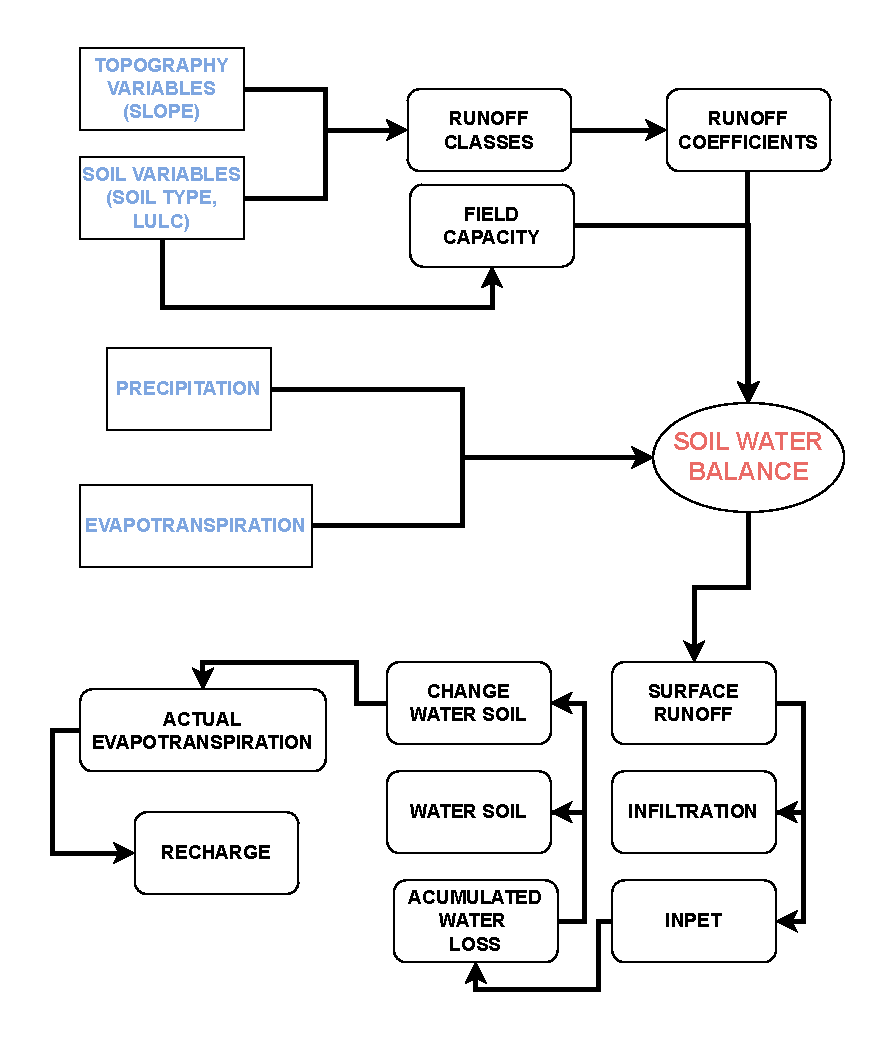
\includegraphics[scale=0.6]{methodology.pdf}
	\caption{Methodology.}\label{fig:methodology}
\end{figure}

\subsection{Soil Water Balance}


The soil water balance for a raster cell at a given month $i$ is given by:
\begin{equation}
P_{i}=R_{i}+AET_{i}+CWS_{i}+REC_{i}
\end{equation}
where
\begin{itemize}
\item $P_{i}$ is the precipitation 
\item $AET_{i}$ is the actual evapotranspiration
\item $CWS_{i}$ is the change in the water stored in the soil
\item $REC_{i}$ is the recharge
\end{itemize}
The surface runoff is calculated using the rational approach as the product of the runoff coefficients and the precipitation:
\begin{equation}
R_{i}=RC \times P_{i}
\end{equation}
where $RC$ is the runoff coefficient which depends on the soil type and use, and slope. 

The infiltration is the difference between the precipitation and the surface runoff:
\begin{equation}
IN_{i}=P_{i}-R_{i}
\end{equation}

The difference between infiltration and potential evapotranspiration is called IN-PET
\begin{equation}
INPET_{i}=IN_{i}-PET_{i}
\end{equation}
A positive INPET indicates a potential accumulation of water in the soil, whereas  the soil is drying if the INPET is negative. 

The accumulated water loss is the sum of the negative values of the INPET since the beginning of the year:
\begin{equation}
AWL_{i}=\sum\limits_{j=0}^{i}\text{NEG}(INPET_{j})
\end{equation}
The water stored in the soil can be calculated as follows:
\begin{equation}
WS_{i}=\left\{
\begin{aligned}
	&FC \times 10^{(b \times INPET_{i})} &\text{If } INPET_{i} < 0 \\
	&WS_{i-1} & \text{If } INPET_{i} > 0
\end{aligned}
\right.
\end{equation}
where
\begin{equation}
b=\frac{0.455}{FC}
\end{equation}
and $FC$ is the field capacity

The change in water storage is the difference between the water stored for a given month and the water stored in a previous month:
\begin{equation}
CWS_{i}=WS_{i}-WS_{i-1}
\end{equation}

There is actual evapotranspiration if  INPET is positive, that, is, the infiltration exceeds the potential evapotranspiration:
$$
AET_{i}=\left\{
\begin{aligned}
	&PET_{i} &\text{If } INPET_{i} \ge 0 \\
	&PET_{i}+[INPET_{i}-CWS_{i}] &\text{If } INPET_{i} < 0 \\
\end{aligned}
\right.
$$

The recharge can be calculate as follows:
$$
REC_{i}=\left\{
\begin{aligned}
	&INPET_{i}-CWS_{i} &\text{If } INPET_{i}>0\\
	&0 &\text{If } INPET_{i}<0\\
\end{aligned}
\right.
$$
\subsection{Input Data}

\subsubsection{Soil Information}

Soil type and Soil use (see Figure \ref{fig:soil})

\begin{figure}
	\centering
	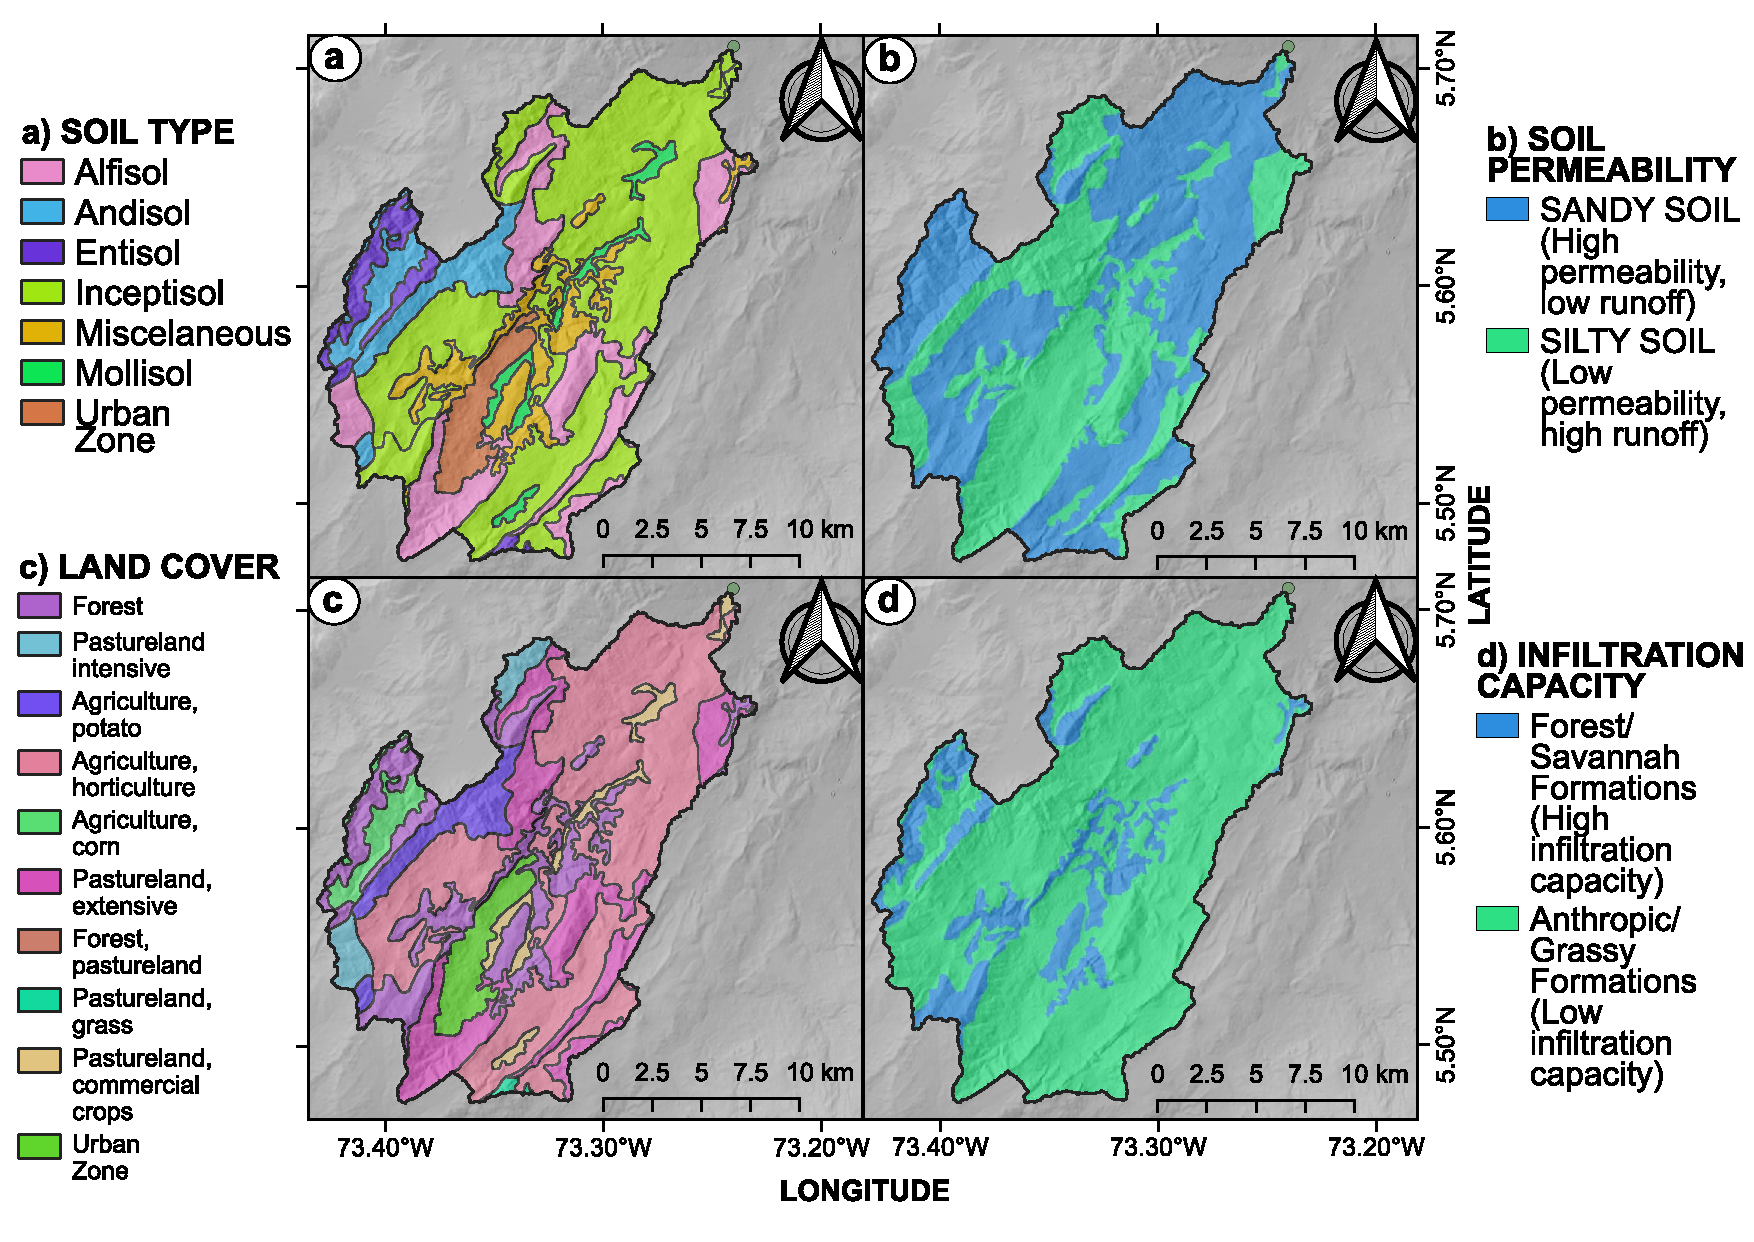
\includegraphics[scale=0.5]{Soil_variables1_Optimized.pdf}
	\caption{Soil information. a) Soil type. b) Soil permeability, c) Land use and land cover, d) Infiltration capacity.}\label{fig:soil}
\end{figure}

\subsubsection{Slope}



\begin{figure}
	\centering
	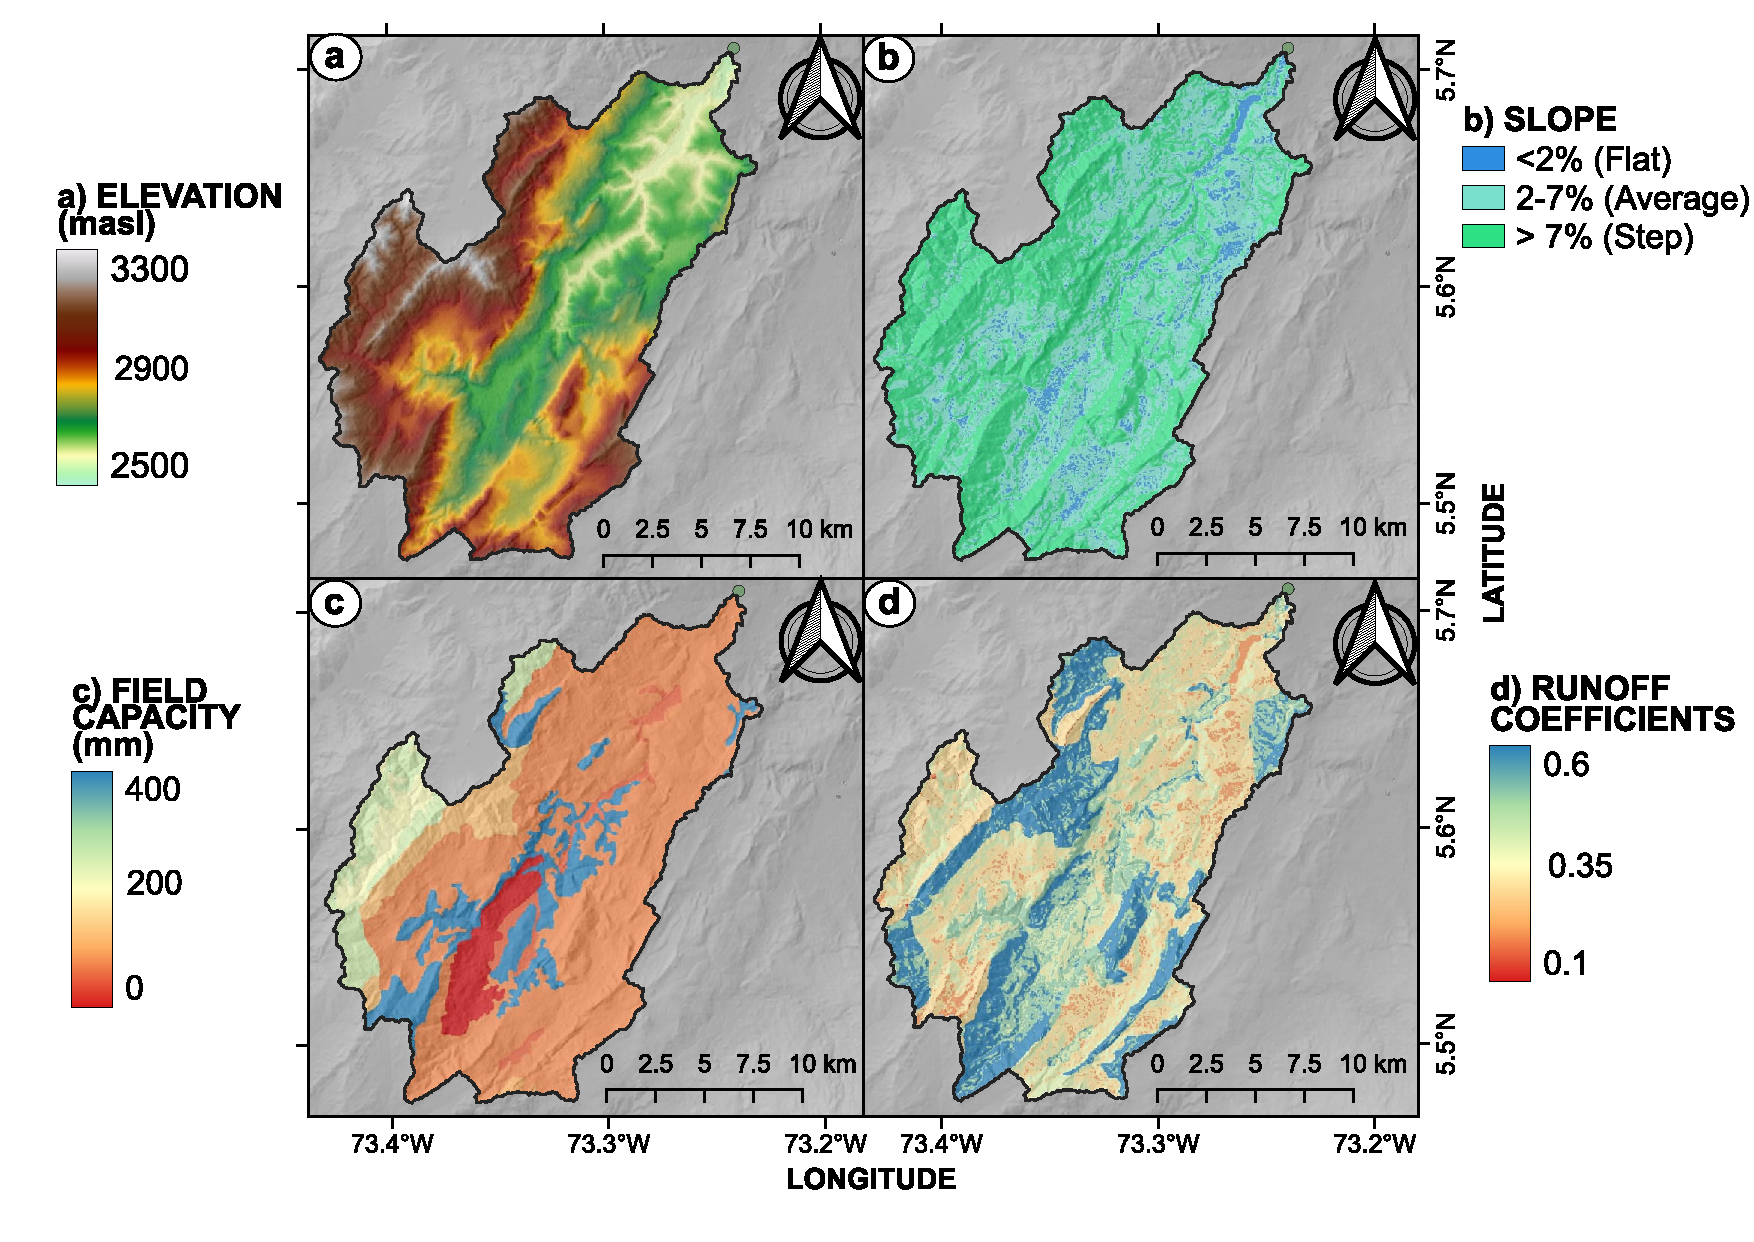
\includegraphics[scale=0.5]{Input_variables2_Optimized.pdf}
	\caption{Slope, Field Capacity and runoff coefficients.}
\end{figure}


\subsubsection{Precipitation}

\begin{figure}
	\centering
	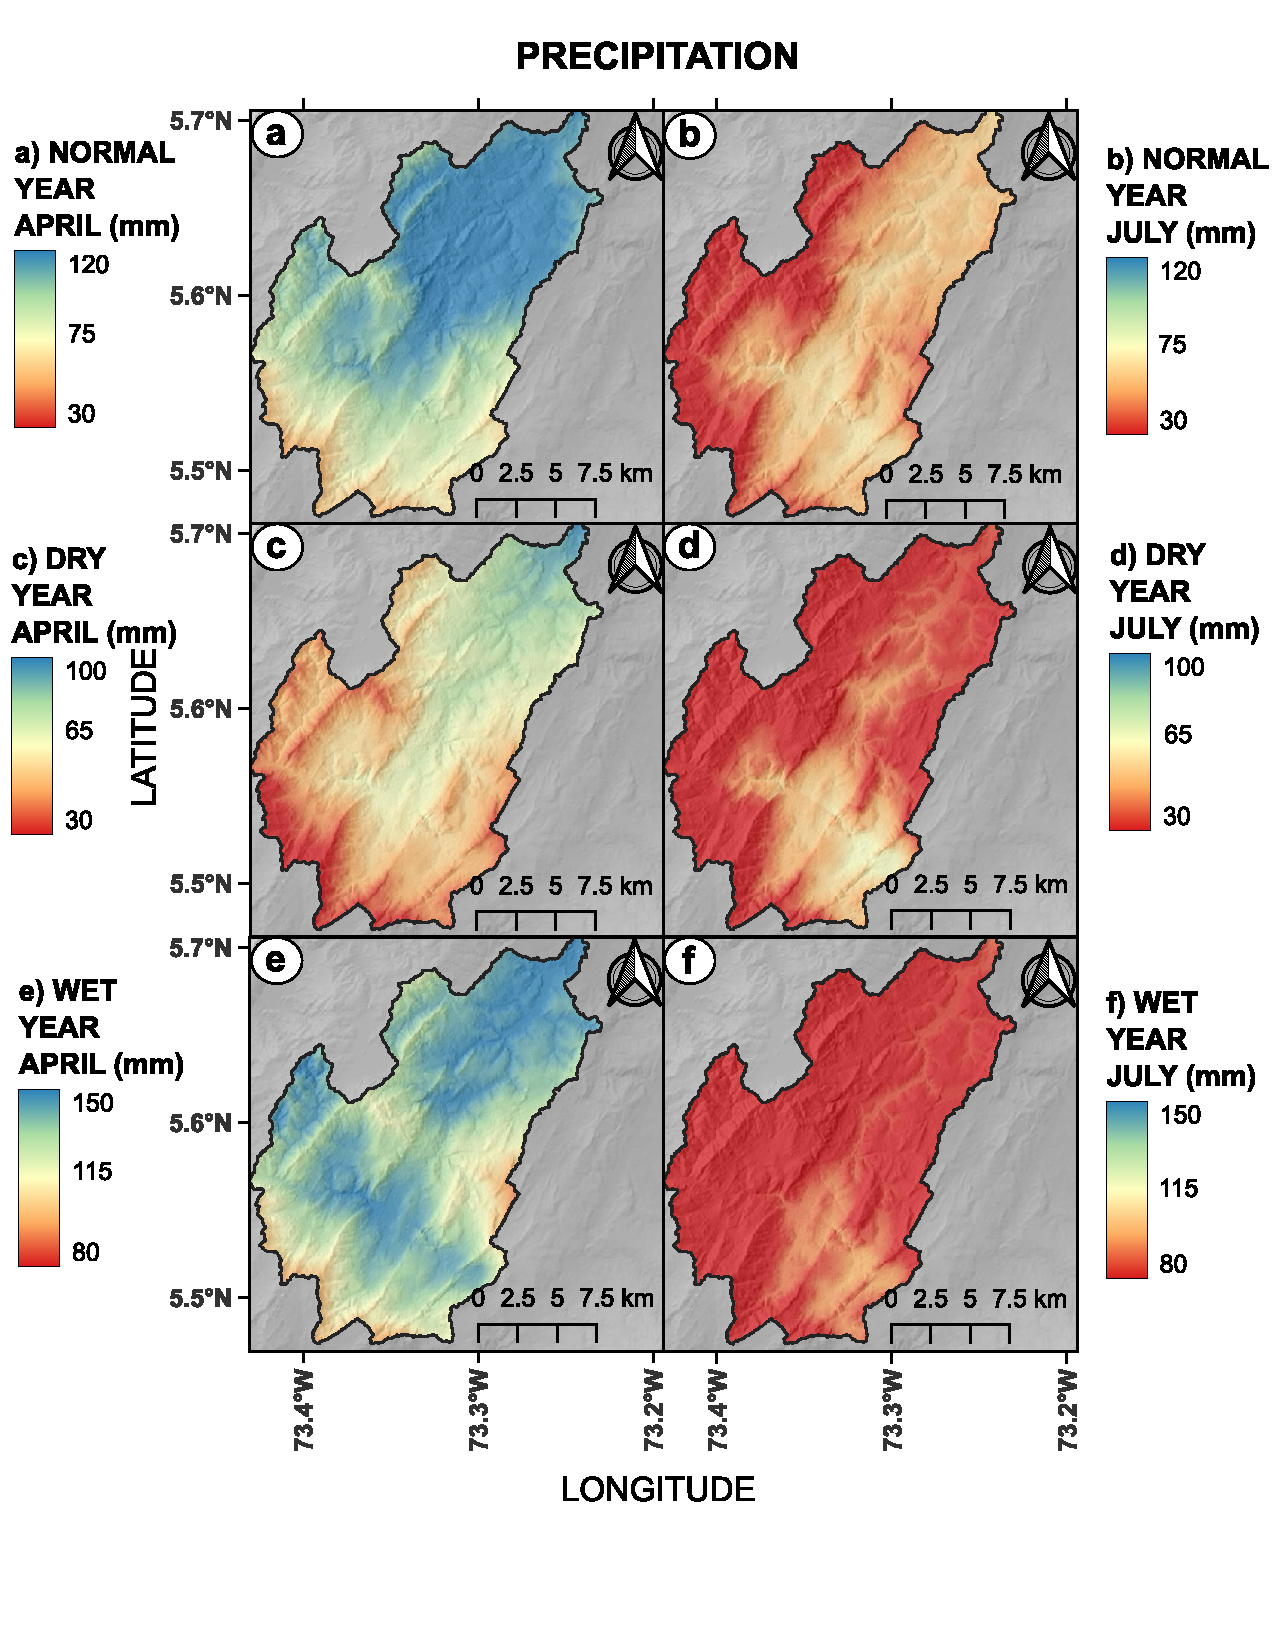
\includegraphics[scale=0.6]{precipitation1_Optimized.pdf}
	\caption{Precipitation}
\end{figure}
	

\subsubsection{Potential Evapotranspiration}


\begin{figure}
	\centering
	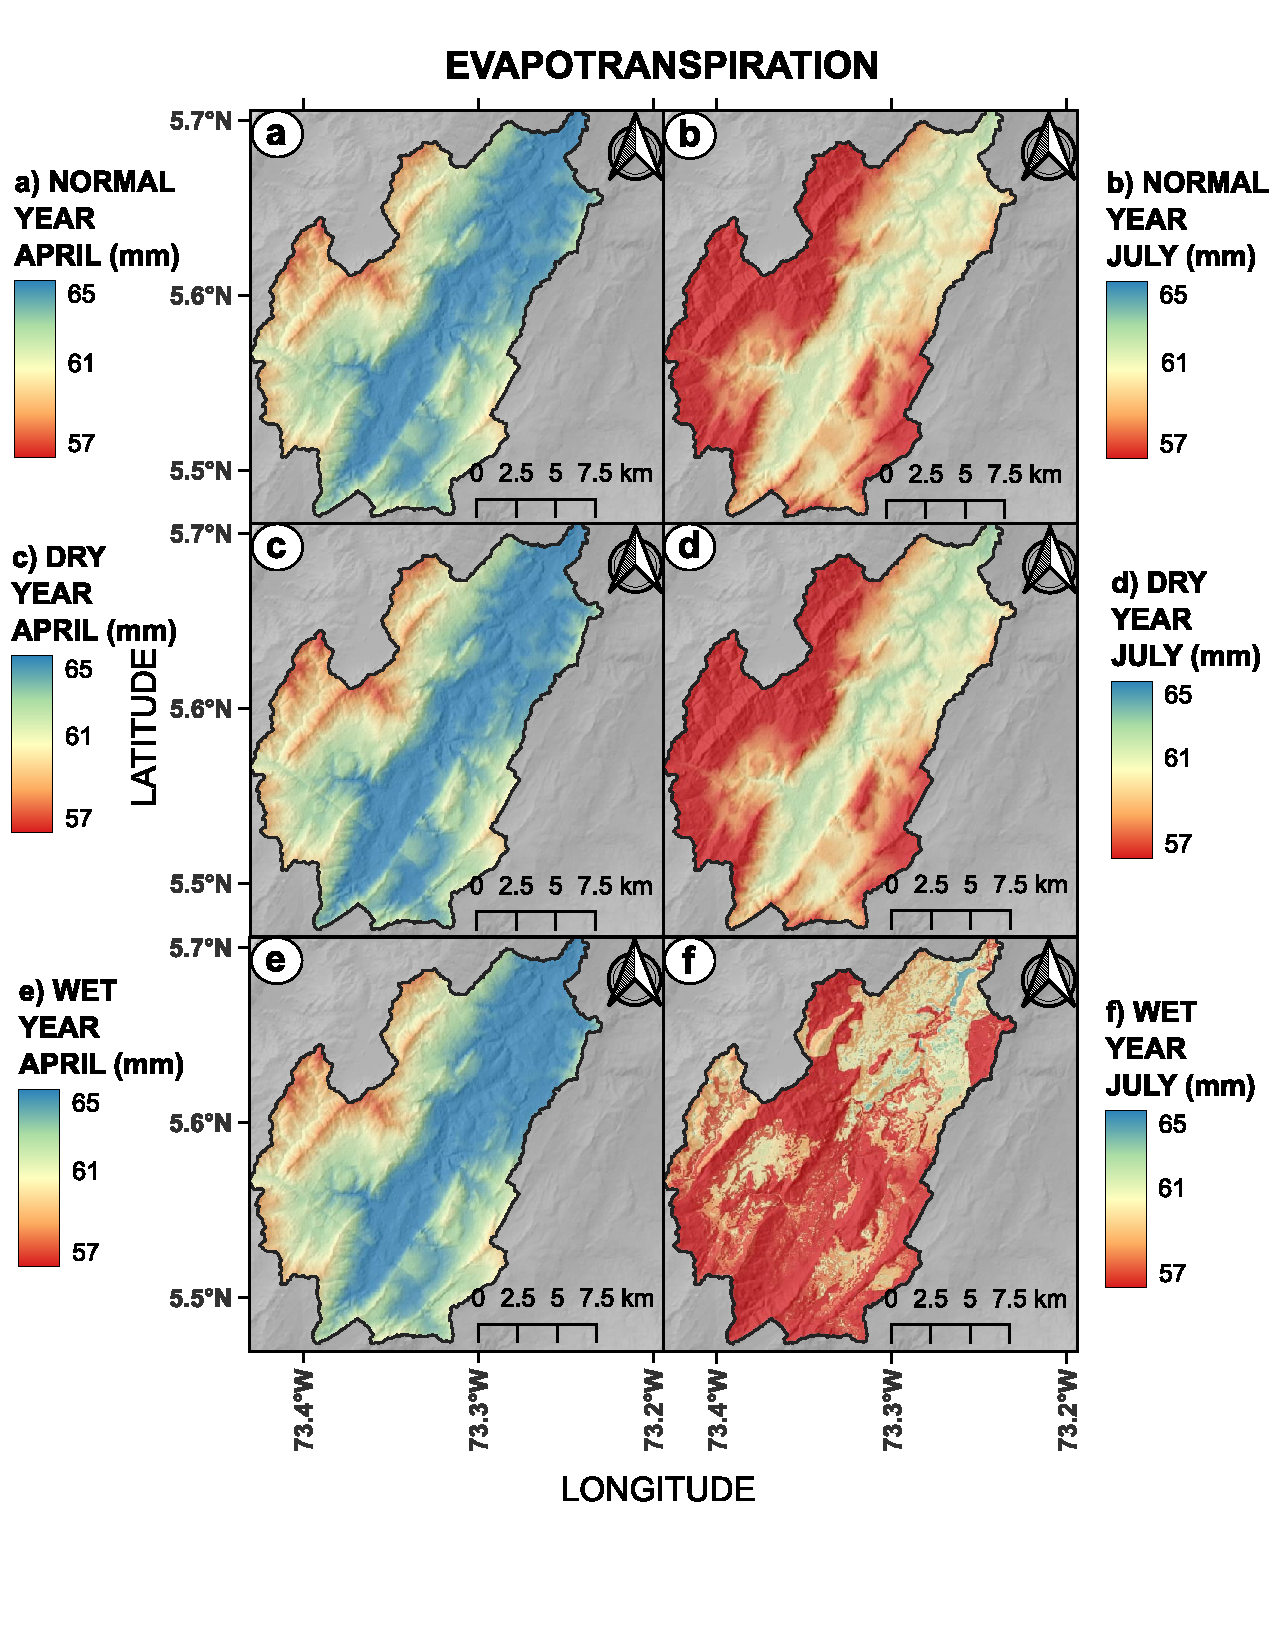
\includegraphics[scale=0.6]{evt_Optimized.pdf}
	\caption{Evapotranspiration}
\end{figure}

%%%%%%%%%%%%%%%%%%%%%%%%%%%%%%%%%%%%%%%%%%%
\section{Results}

\subsection{General}



Figure \ref{fig:recharge_annual} shows the results of the annual recharge estimated for the study area for normal, dry and wet years.  

\begin{figure}
	\centering
	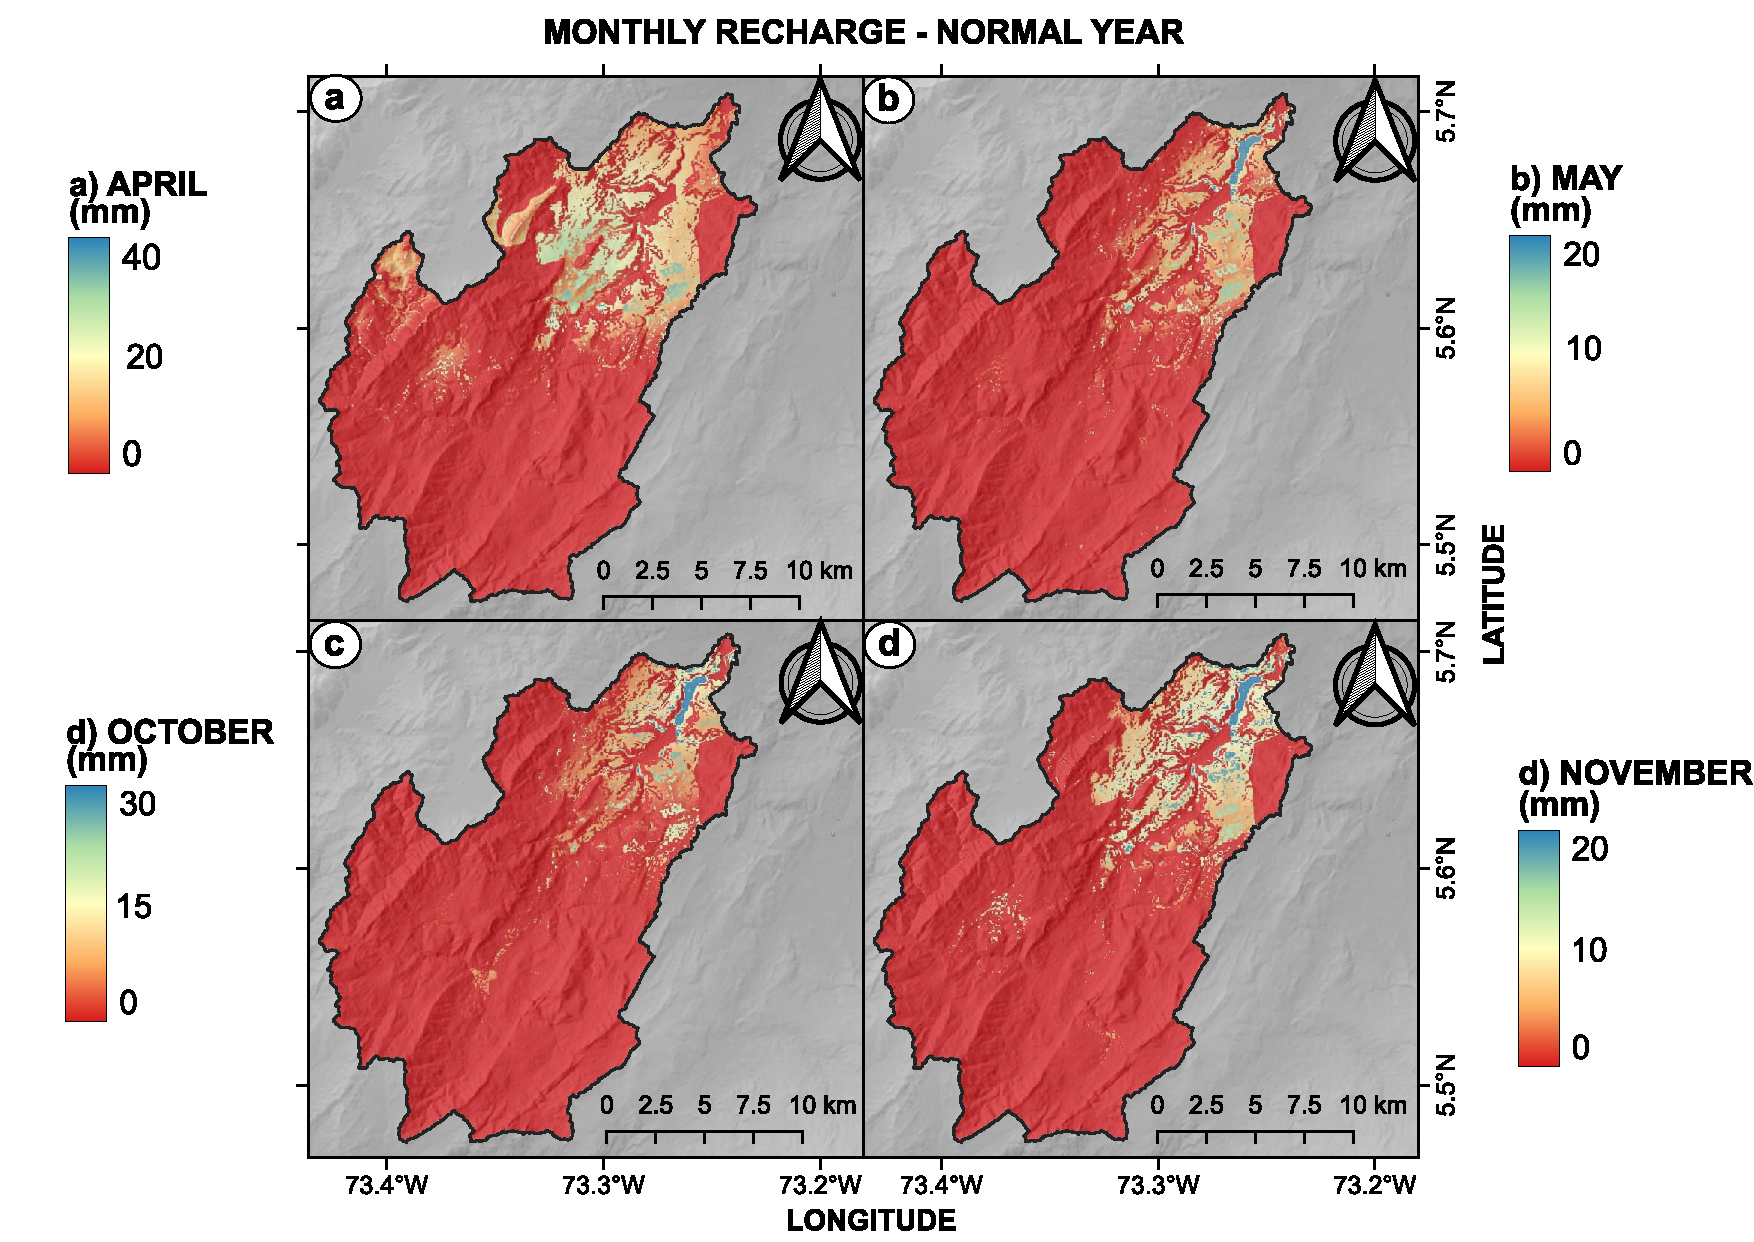
\includegraphics[scale=0.5]{montly_recharge_normal_Optimized.pdf}
	\caption{Monthly recharge normal year.}\label{fig:recharge_normal}
\end{figure}

\begin{figure}
	\centering
	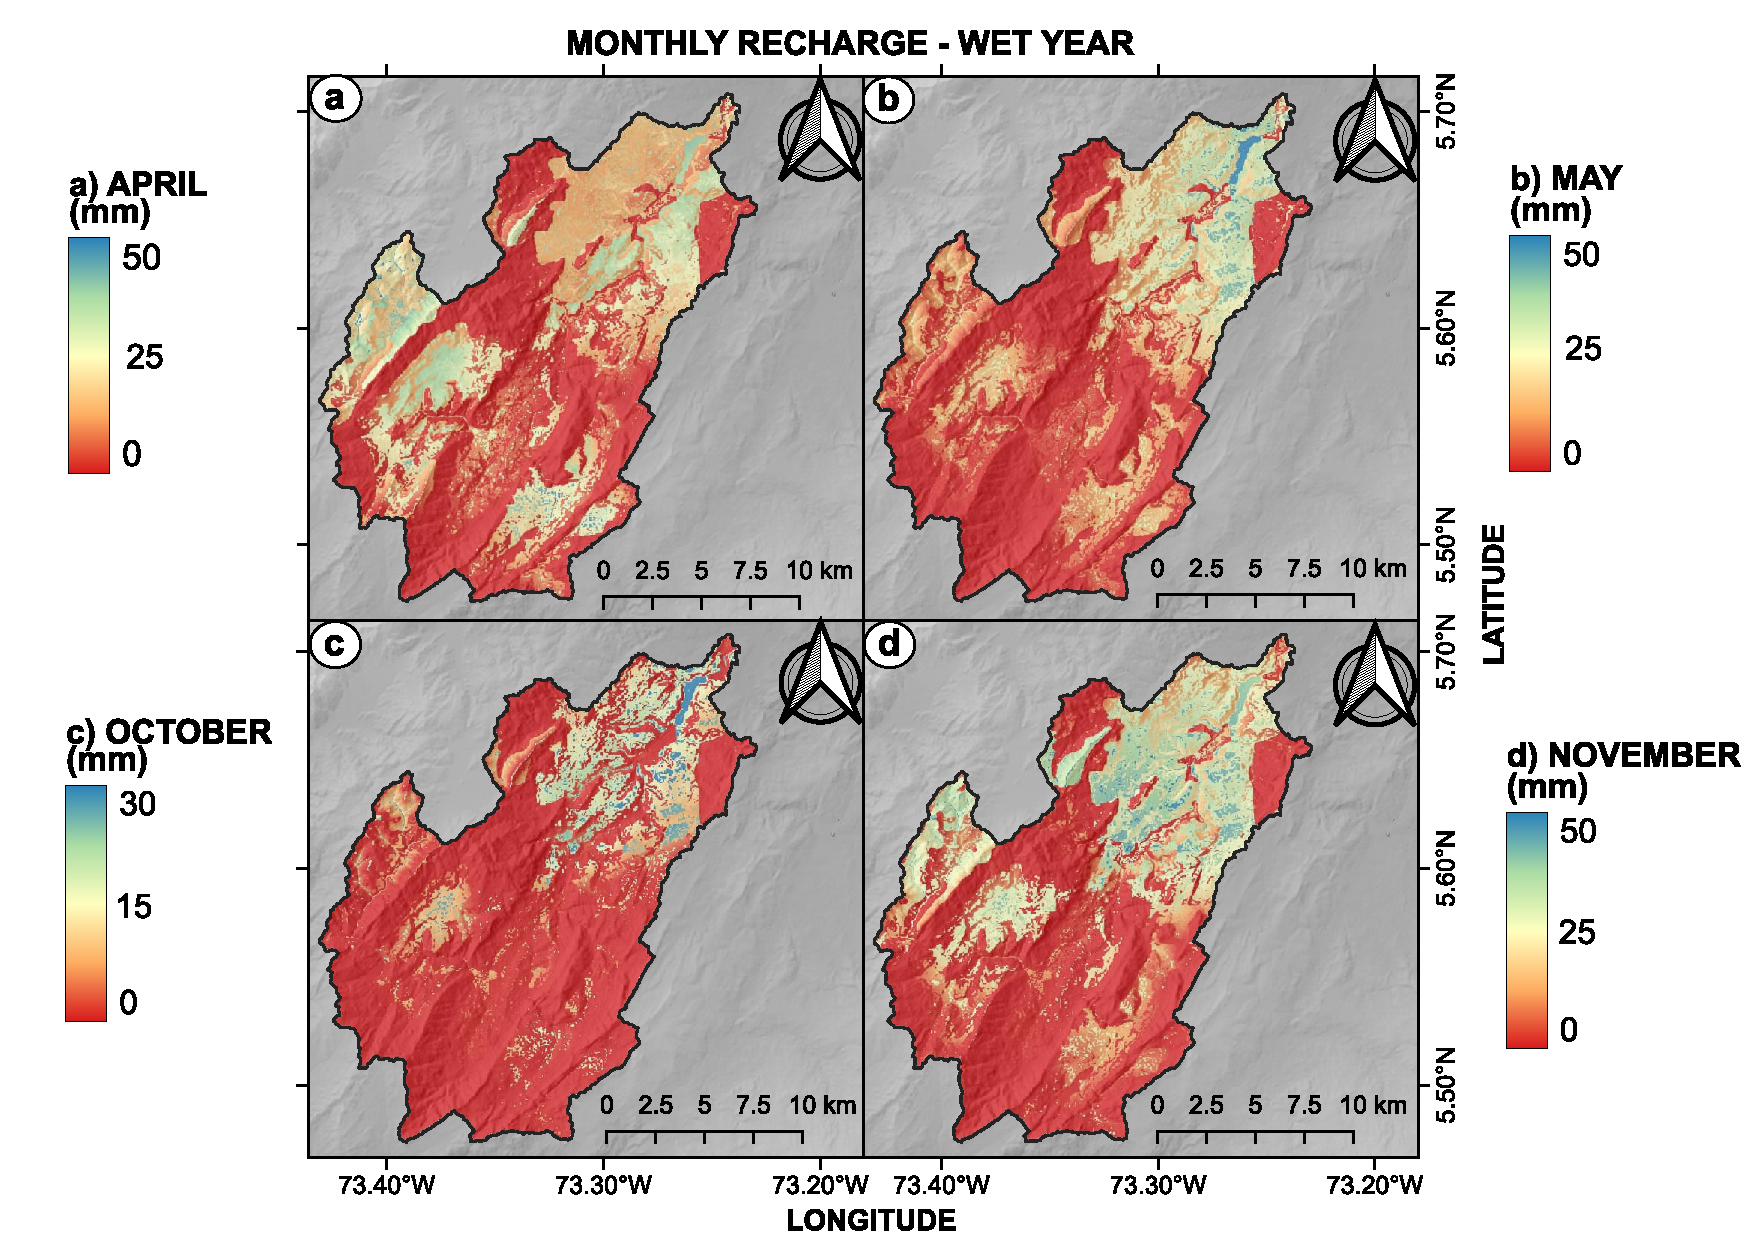
\includegraphics[scale=0.5]{montly_recharge_wet_Optimized.pdf}
	\caption{Monthly recharge wet year.}\label{fig:recharge_normal}
\end{figure}


\begin{figure}
	\centering
	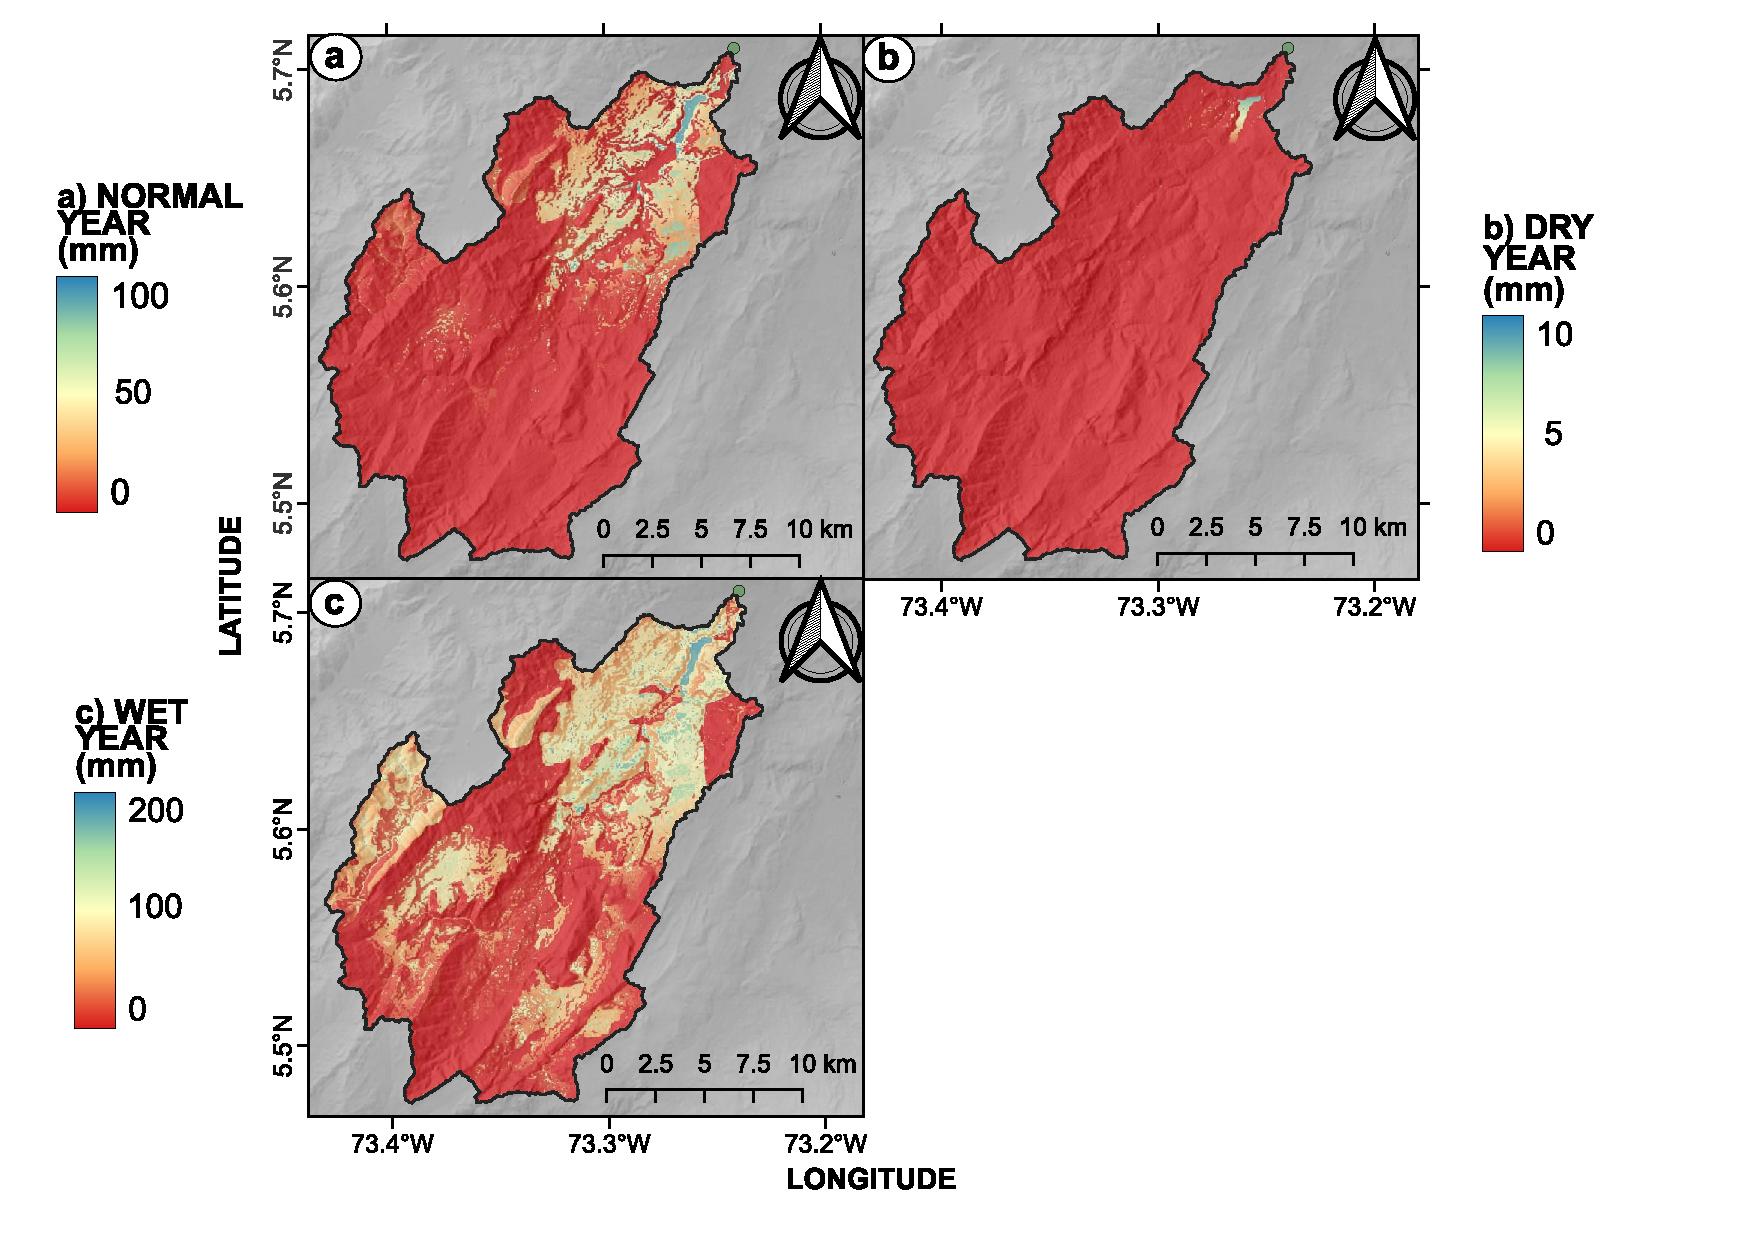
\includegraphics[scale=0.5]{recharge_Optimized.pdf}
	\caption{Annual recharge in the Vega River watershed obtained using the soil water balance approach. a) Annual recharge for a normal year, b) Annual recharge for a dry year, c) Annual recharge for a wet year. CALCULATE STATISTICS?. }\label{fig:recharge_annual}
\end{figure}


\subsection{Water balance by Runoff Classes}

\subsection{Water balance by Land Use Classes}

\subsection{Water Balance by Geological Unit}

%%%%%%%%%%%%%%%%%%%%%%%%%%%%%%
\section{Discussion}

\begin{itemize}
	\item Answer Research Questions. Defend Answer with Results
	\begin{itemize}
		\item Q1: Magnitude (annual recharge). 
		%Results shown in Figure \ref{fig:recharge_annual} indicate that groundwater recharge heavily depends  on the amount of precipitation over the study area. There is only \SI{10}{\milli \meter} of recharge to the aquifer in the north part of the study area during the dry years (see Fig. \ref{fig:recharge_annual}b), and there is no recharge in the aquifers located near the city of Tunja (SW part of the study area). 
		%During a normal year, the annual recharge ranges between \qtyrange{50}{100}{\milli \meter} in the NE part of the study area in the Tilat� Fm and Quaternary deposits in Tuta municipality and in the Guaduas, Bogot� and Tital� Formations in Combita municipality, respectively.  The  annual recharge increases to \qtyrange{100}{200}{\milli \meter}.
		
		From the results, there are second recharge zones located in the study area. The first area called NE recharge area is located in the Tuta and Combita municipalities (see Fig. location) and it is characterized by annual recharges between \qtyrange{50}{100}{\milli \meter} during the normal years that increases to  \qtyrange{100}{200}{\milli \meter}  during wet years. The aquifers associated with this recharge zone include confined aquifers of the Tilata Fm and phreatic to locally confined aquifers in the Quaternary deposits.
		
		The second recharge area is located near Tunja municipality (capital of Boyaca state) and it is characterized by annual recharges between \qtyrange{20}{130}{\milli \meter} during the wet years with nill recharge during the dry and normal years. The aquifers associated with this recharge zones mainly include confined aquifers of the Bogota Formation.
		
		
		
		    
		\item Q2: Places where recharge is high/low
		\item Q3: Months where recharge is high. 
	\end{itemize}
	\item Explain
	\begin{itemize}
		\item Conflicting results
		\item Unexpected findinds
		\item Discrepancies with other research
	\end{itemize}
	\item Limitations
	\item Importance
	\item Newness
\end{itemize}
%%%%%%%%%%%%%%%%%%%
\section{Conclusions}

%%===========================================================================================%%
%% If you are submitting to one of the Nature Portfolio journals, using the eJP submission   %%
%% system, please include the references within the manuscript file itself. You may do this  %%
%% by copying the reference list from your .bbl file, paste it into the main manuscript .tex %%
%% file, and delete the associated \verb+\bibliography+ commands.                            %%
%%===========================================================================================%%

\bibliographystyle{model3a-num-names}
\bibliography{GWRechargeRioJordan}% common bib file
%% if required, the content of .bbl file can be included here once bbl is generated
%%\input sn-article.bbl


\end{document}
